\renewcommand{\figurename}{}
\mychapter{R4Cyber.09 Sécurité des Réseaux LAN (16h30)}{cap:r4c09} 
\lhead{R4Cyber.09 Sécurité des Réseaux LAN (16h30)}

\vspace*{0.2cm}%
      \large
      \href{}{\color{black}Enseignant\\M. Laurent Gallon}\\%
      \normalsize
\vspace*{0.5cm}%

Ce module portait sur la sécurisation des réseaux locaux d'entreprise. Dans celui-ci, nous avons revu le fonctionnement de protocoles réseaux utilisés dans les réseaux locaux d'entreprise, pour ensuite en voir une application utilisée pour des attaques courantes les utilisant.
\\ \\
Pour se prémunir de ces attaques et mieux les comprendre, nous les avons expérimentées dans des environnements contrôlés, puis nous avons mis en place des mécanismes de protection pour s'en prémunir.

\section{Forger des paquets volontairement malicieux sur un réseau}

% forger ses paquets avec scapy

Pour simuler les attaques, nous avons appris à initier un comportement anormal sur un réseau en modifiant les informations que l'on envoie sur celui-ci.
\\ \\
Notre intention dans une attaque est de générer un comportement anormal sur une machine ciblée. Pour ce faire, nous devions forger des demandes malicieuses pour provoquer une réaction attendue chez elle.
\\ \\
Nous avons donc appris à utiliser l'outil \texttt{Scapy} pour générer tout type de trafic réseau, en modifiant à souhait la composition de nos demandes. Nous pouvions notamment à l'issue usurper l'identité d'un hôte sur le réseau pour que celui-ci reçoive des communications que nous avions initiées à sa place.

\section{Prise en main des attaques courantes}

Suite à cet apprentissage, nous avons pu commencer notre étude des attaques étudiées théoriquement. Nous en avons notamment montées deux : l'attaque de l'homme du milieu par empoisonnement de la table ARP, et l'attaque du déni de service par rebond. Je vais en présenter une ici.

\subsection{Attaque de l'homme du milieu par empoisonnement ARP}

% mitm par arp poisoning

Pour la première, il nous fallait revoir le fonctionnement du protocole ARP. Celui-ci est indispensable pour utiliser le protocole IPv4, servant à trouver qui possède une adresse IP dans un réseau local.
\\ \\
Notre objectif, côté attaquant, fut de dire dans un réseau local à toutes les machines que nous étions maintenant leur passerelle, ou leur "box". Nous disions à haute voix notre nouvel emplacement pour usurper identité de la vraie passerelle, afin que les machines pensent que si elles veulent accéder à Internet, qu'elles le fassent par nous.
\\ \\
Nous avions par la suite qu'à renvoyer les demandes de connexion vers la vrai passerelle, et renvoyer les réponses aux victimes. Nous pouvions donc voir les connexions que les machines effectuées sur Internet, et si non protégées : voir leur contenu.

\begin{figure}[H]
    \centering
    \captionsetup{justification=centering}
    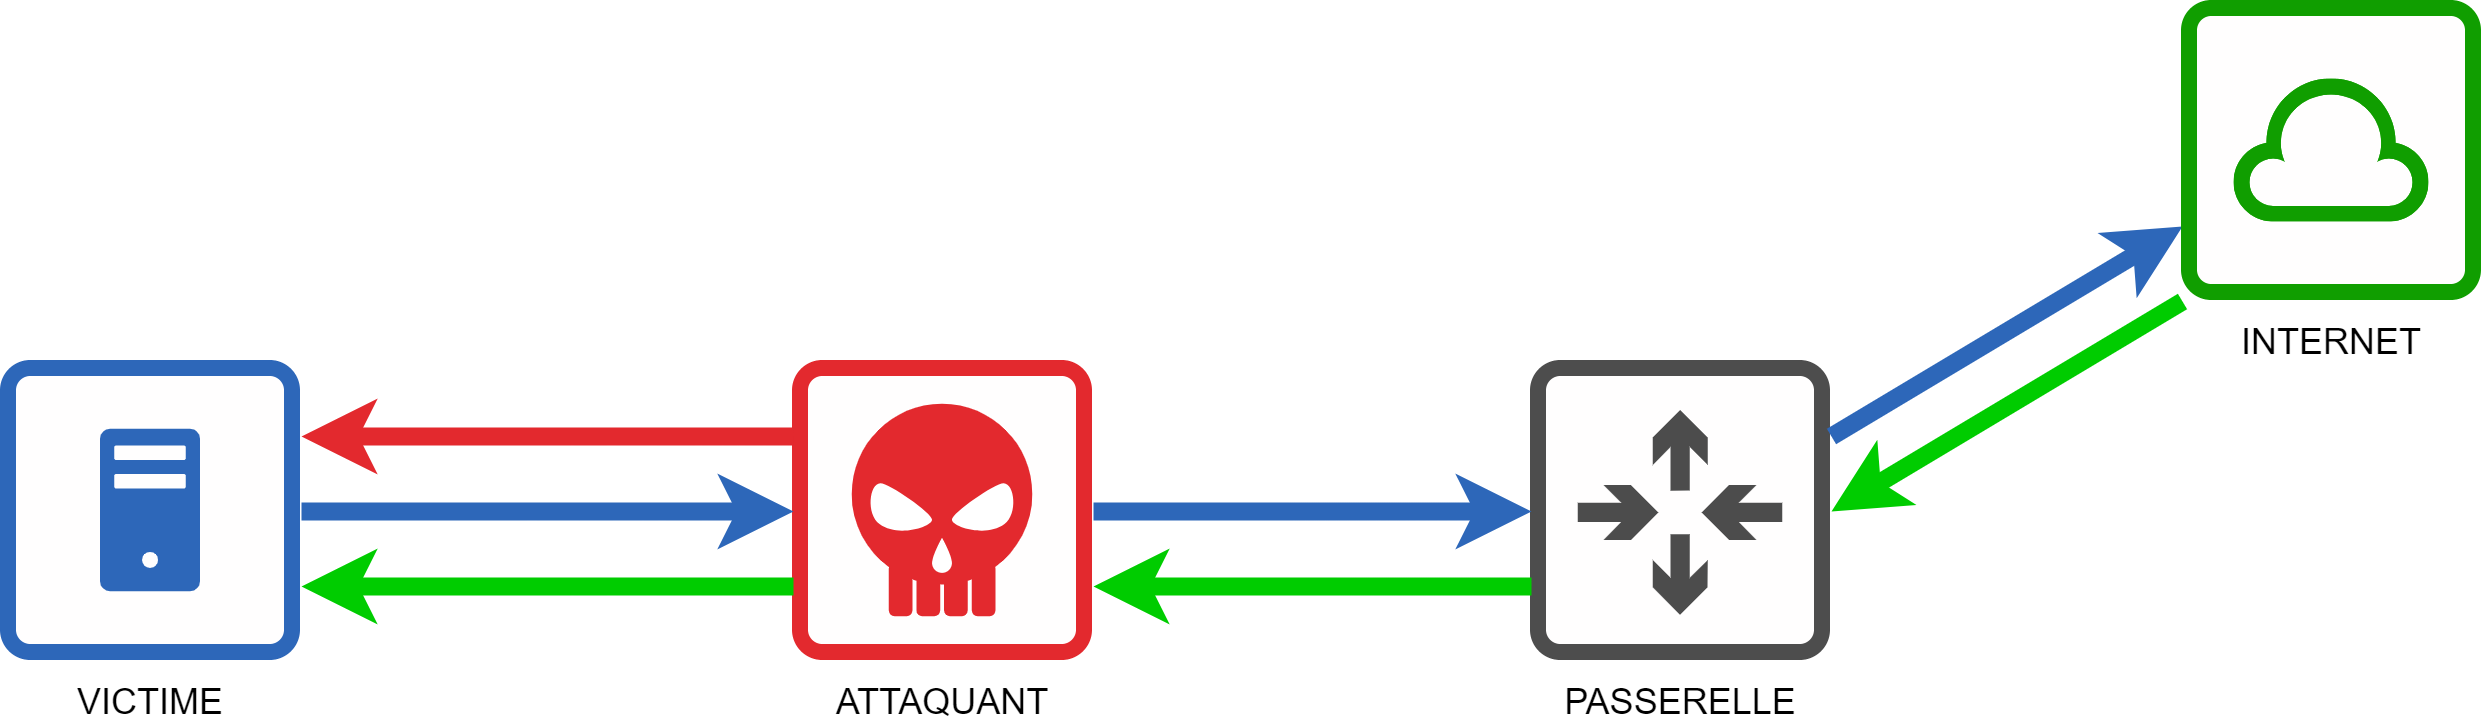
\includegraphics[width=\textwidth - \textwidth / 20]{ressources/arp_poisoning_2.png}
    \figurename
    \caption{Illustration de l'attaque par l'homme du milieu par empoisonnement de table ARP. L'attaquant informe qu'il est le nouvel emplacement de la passerelle du réseau pour intercepter les requêtes et les réponses attendues pour la victime.}
    \label{fig:poste}
\end{figure}

% icmp smurf (ip source = victime, ip dest. = broadcast)
